We now have enough methods to begin approximating both the particle system and the kinetic model. As in previous sections, we first focus on the particle system, before involving the continuum approach. 
\subsection{Space-Homogeneous Particle Model}\label{sec:homparticles}
Recall the homogeneous particle model \eqref{eq:homparticle},
\begin{equation}\tag{\ref{eq:homparticle}}
\dif v^{i,N}_t = G\left(\frac{1}{N}\sum_{j=1}^n v^{j,N}_t\right)\dif t-v^{i,N}_t \dif t + \sqrt{2\sigma} \dif W^i_t.
\end{equation}
Simulating this system is analagous to solving the Ornstein-Uhlenbeck process of Section \ref{sec:particlemethods}. The interaction term is easily calculable using NumPy's \texttt{mean()} function as it is simply the average velocity of all the particles at each time step. The Euler-Maruyama scheme for this system is
\[ v^{i,N}_{n+1} = v^{i,N}_n - v^{i,N}_n\Dt + G\left(\frac{1}{N}\sum_{j=1}^N v^{j,N}_n\right)\Dt+ \sqrt{2\sigma\Dt} Z^i_n. \]
As the system contains interactions, simulating one particle for a long time is no longer sufficient. Multiple particles must be simulated simultaneously. Figure +++ref++ shows 
\begin{figure}
    \centering
    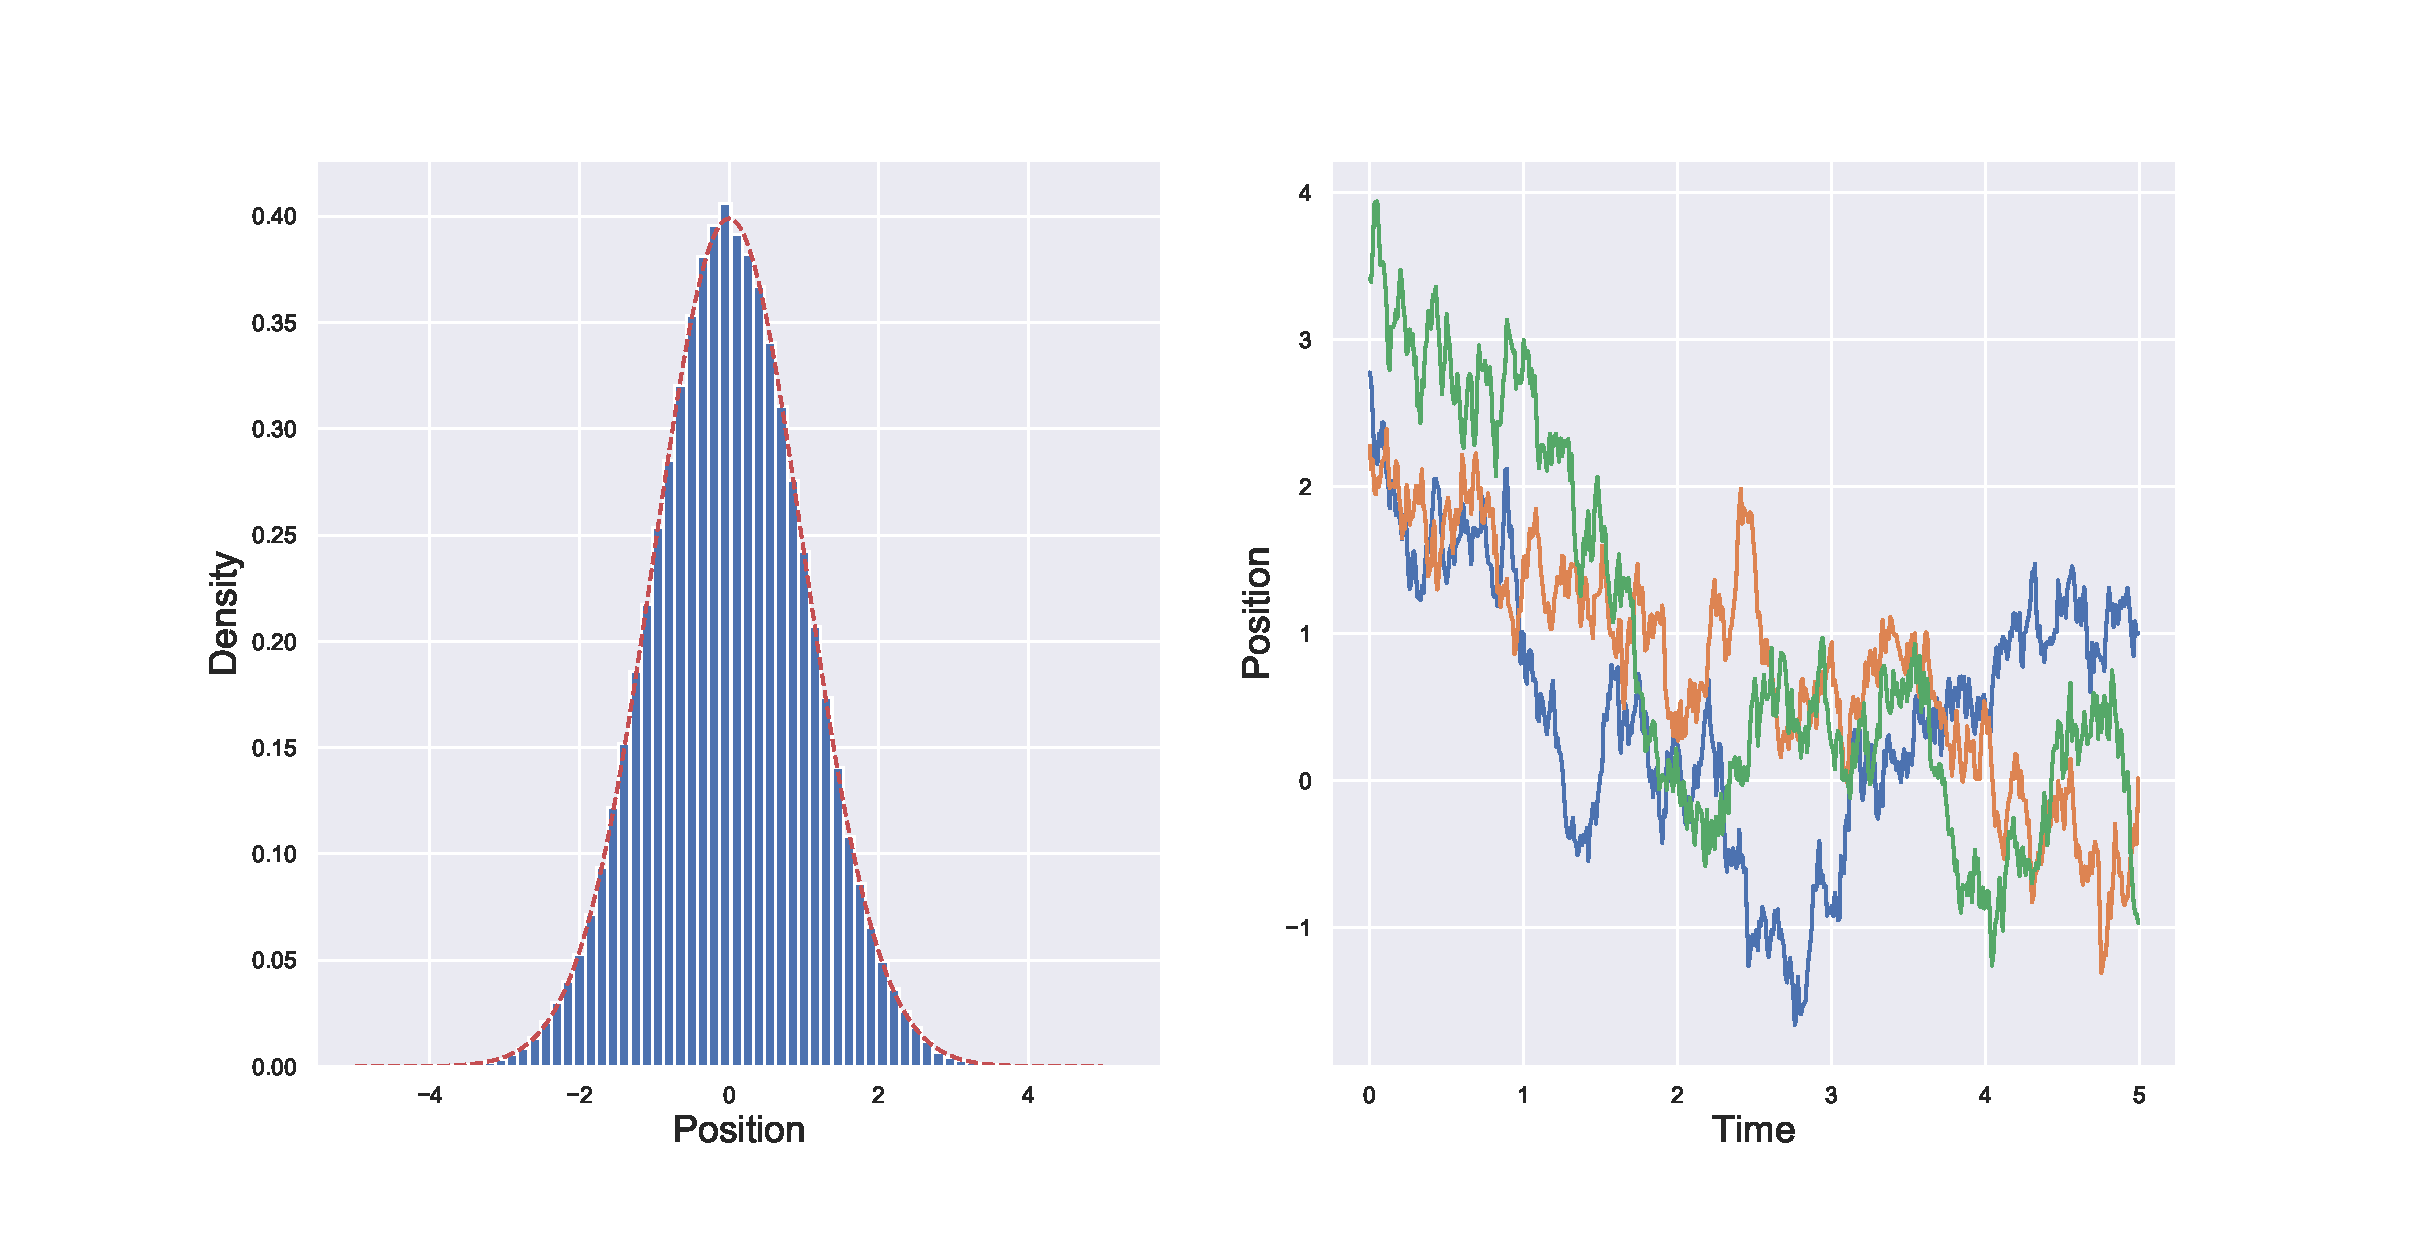
\includegraphics[width=0.7\linewidth]{Figures/OUparticletraj}
    \caption{Histogram of positions of 1000 particles after 100s with $\sigma = 1$, and positions of 5 particles over time. +++conv in moments?+++}
    \label{fig:ouparticletraj}
\end{figure}

\subsection{Space-Homogeneous Kinetic Model}\label{sec:homkin}
 Consider the space-homogeneous evolution given by \eqref{eq:spacehomPDE}, that is
    \begin{equation}
    \partial_t f_t(v) = \partial_v vf_t(v) - \partial_v G(\langle w \rangle_{f_t})f_t(v) + \sigma \partial_{vv} f_t(v).
    \end{equation}
    Using the methods developed in the previous section, we are now able to solve this system numerically. As when solving the heat equation, a zero boundary condition shall be enforced. This is valid as we know that the stationary distributions are Gaussian and centred at $-1,0,+1$. The boundary $L$ can then be chosen depending on the the diffusion so that almost no mass is contained beyond the boundary. For example if $\sigma = 1$, the mass contained beyond $L=5$ is of the order $10^{-5}$. 
    
    Simpson's rule will be used as a quick way to approximate the integral within the herding coefficient. To differentiate between the integral and its approximation, we write \(\langle w\rangle_{F^n}\). Below is the scheme when both the herding coefficient and the velocity are positive, using a finite difference scheme with a CN discretisation for the diffusive term and an upwind method for the damping and herding terms.
    \begin{equation*}
    \begin{split}
    \frac{F_j^{n+1} - F_j^n}{\Delta t} = 	-G(\langle w\rangle_{F^n})\left[ \frac{F^n_{j+1} - F^n_{j}}{\Delta v}\right] &+\left[ \frac{v_{j}F^n_{j} - v_{j-1}F^n_{j-1}}{\Delta v}\right]\\ &+ \frac{\sigma}{2}\left[ \frac{F^{n+1}_{j+1} - 2F^{n+1}_j + F^{n+1}_{j-1}}{(\Delta v)^2} + \frac{F^{n}_{j+1} - 2F^{n}_j + F^{n}_{j-1}}{(\Delta v)^2}\right] 	 
    \end{split}
    \end{equation*}
    
    +++Pictures, moments converging, error (in moments too?) in particular, mass loss? -> compare conservative methods i.e. fin vol +++
\subsection{Space-Heterogeneous Particle Model}\label{sec:hetkin}
    +++ phi = 1 still, moving in space. Animations/diagrams showing Leb in space. +++
    